\section{Introduction to representability}

%This chapter will introduce definitions and results that are necessary to discuss the representability.
%
%More specifically, this chapter will introduce:
%\begin{itemize}
%\item Why we care about representability
%  \begin{itemize}
%  \item If all matroids are representable, we are just giving a vector space another name.
%  \item Therefore, it is important that not all matroids are representable.
%  \item Show some examples of unrepresentable matroids
%  \item Now that we know the existence, the question is, which one?
%  \end{itemize}
%\item The mathematical definition of "representability"
%\end{itemize}

We will start this chapter by defining the representability of a matroid.

\begin{defn}
A matroid $M = (E, \mathcal{I})$ is representable over a field $\mathbb{F}$ if 
there exists a matrix $A$ over $\mathbb{F}$ such that the column matroid of $A$ is isomorphic to $M$.
\end{defn}

The representability is an important and interesting part of the matroid theory.
For example, if there exists a field $\mathbb{F}$ such that all matroids are representable over $\mathbb{F}$,
the matroid theory did not quite succeed in abstracting the concept of linearly independence
as those properties could have been found by studying a set of vectors over $\mathbb{F}$.
Fortunately, a lot of unrepresentable matroids have been found including V\'{a}mos matroid which is not representable over any field. \cite{matroidtheory}

Before introducing some more unrepresentable matroids, we will start by introducing a nice property of representable matroids.

\begin{thm}
Let $M = (E, \mathcal{I})$ be a matroid that is representable over $\mathbb{F}$.
Let $r$ be a rank of $M$ and $k = \lvert E \rvert$.
Then there exists a matrix $A \in \mathbb{F}^{r \times k}$ such that $M$ is isomorphic to the column matroid of $A$.
\end{thm}

\begin{proof}
Let $B$ a matrix over $\mathbb{F}$ such that the column matroid of $B$ is isomorphic to $M$.
It is easy to see that the number of columns of $B$ is $k$.
From linear algebra, we know that elementary row operations preserve the linear independence of column vectors.
Let $R$ be the reduced row echelon form of $B$.
Since $R$ must have a rank of $r$, $R$ has exactly $r$ non-zero row vectors.
Removing zero rows clearly does not affect the linear independence.
Therefore, we found a matrix in $\mathbb{F}^{r \times k}$ whose column matroid is isomorphic to $M$.
\end{proof}

This property is useful when proving that a matroid is unrepresentable over some field.

Here are some matroids that are not representable over some fields.

\begin{thm}
$U_{2, 4}$ is not representable over $GF(2)$.
\end{thm}

A matroid is called a \textit{binary matroid} if it is representable over $GF(2)$.

\begin{proof}
We know that $U_{2, 4}$ has a rank of $2$.
If $U_{2, 4}$ is representable over $GF(2)$, there exists a matrix $A \in GF(2)^{2 \times 4}$ such that $A$'s column matroid is isomorphic to $U_{2, 4}$.
Since $GF(2)$ only has two elements, there are only four possible column vectors of size 2.
$\bigg\{\begin{pmatrix}0\\0\end{pmatrix},
\begin{pmatrix}0\\1\end{pmatrix},
\begin{pmatrix}1\\0\end{pmatrix},
\begin{pmatrix}1\\1\end{pmatrix}\bigg\}$
$A$ must not contain $\begin{pmatrix}0\\0\end{pmatrix}$ since it is a loop. 
Since $A$ has 4 columns and there are only 3 different column vectors, we know that there are two columns in $A$ that have the exact same column vector.
This is a contradiction since a subset of such two elements will not be independent.
Therefore, $U_{2, 4}$ is not representable over $GF(2)$.
\end{proof}

\begin{rem}
$U_{2, 4}$ is representable over some field such as $\mathbb{R}$.
For example, the column matroid of $\begin{pmatrix}
1 & 1 & 1 & 1 \\
1 & 2 & 3 & 4 
\end{pmatrix}$ is isomorphic to $U_{2, 4}$.
\end{rem}


Now, we will introduce the Fano matroid.
The Fano matroid can be constructed from the Fano plane.
The Fano matroid is one of the examples of matroids that are representable over $GF(2)$, but not over $\mathbb{R}$.
We will start by defining the Fano matroid mathematically.

\begin{figure}
  \centering
    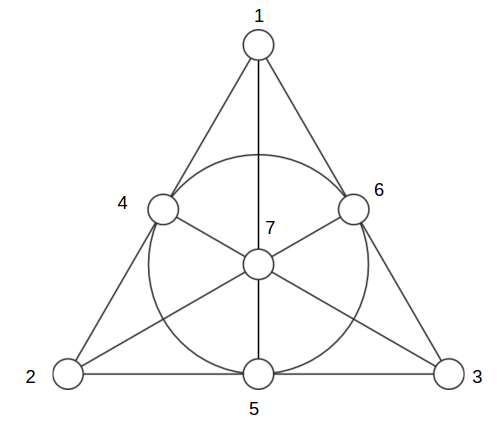
\includegraphics[width=0.8\textwidth,natwidth=610,natheight=642]{Fano_plane.png}
    \caption{Fano plane}
  \label{fig:test}
\end{figure}

\begin{defn}
The Fano matroid is a matroid with a ground set $\{ 1, 2, \cdots, 7 \}$. 
Each number corresponds to the vertex in the figure $1$.
A set $S$ of elements is independent if it satisfies one of the following:
\begin{enumerate}
\item $\lvert S \rvert < 3$,
\item $\lvert S \rvert = 3$ and the corresponding vertices are not on the same line.
\end{enumerate}
$S$ is always dependent if $\lvert S \rvert > 3$.
\end{defn}

For example, $\{4, 5\}$ and $\{ 1, 2, 3 \}$ are independent, but $\{ 1, 4, 2 \}$, $\{1, 5, 7\}$, and $\{4, 5, 6 \}$ are not independent as each of them is on one line.

\begin{thm}
The Fano matroid is indeed a matroid.
\end{thm}

\begin{proof}
An empty set is independent since it contains less than 3 elements.
Any independent set has at most three elements, so any proper subset of it has at most two elements.
Therefore, any subset of independent sets is always independent.
The third property can be proved by checking each case.
Since any set with 2 or fewer elements is independent, we only need to care about the case when we have a set with 2 elements and a set of 3 elements.
Let $A = \{ a_1, a_2, a_3 \}$, $B = \{ b_1, b_2\}$ be independent sets.
It is easy to see from the figure that there must be exactly one line that goes through both $b_1$ and $b_2$.
Let $x$ denote the third point on such line.
Then, adding any element other than $b_1, b_2, x$ to $B$ will generate an independent set of three elements.
Therefore, we just need to make sure that $A \neq \{ b_1, b_2, x \}$.
That cannot be the case since $\{ b_1, b_2, x \}$ is dependent and $A$ is independent.
Therefore, there must be an element $a \in A - B$ such that $B \cup \{ a \}$ is independent.
Since the Fano matroid satisfies all three properties, it is indeed a matroid.
\end{proof}


Here is an interesting property of the Fano matroid
\begin{thm}
If the Fano matroid is representable over a field $\mathbb{F}$, $1 + 1 = 0$ in that field.
\end{thm}

\begin{proof}
Suppose the Fano matroid is representable over a given field $\mathbb{F}$.
Let $A \in \mathbb{F}^{3 \times 7}$ such that $A$'s column matroid is isomorphic to the Fano matroid.
Let $R$ be a reduced row-echelon form of $A$.
Then the first three columns should be identical to $I_3$ since $R$ has a rank of 3.
Since $\{1, 2, 4\}$ is dependent, $R_{3, 4}$ is 0.
Applying the same argument to $\{2, 3, 5\}, \{1, 3, 6\}$, we get the following:\\
$\begin{pmatrix}
1 & 0 & 0 & ? & 0 & ? & ? \\
0 & 1 & 0 & ? & ? & 0 & ? \\
0 & 0 & 1 & 0 & ? & ? & ? \\
\end{pmatrix}$\\
All of $4, 5, 6, 7$th columns have to contain at least two nonzero elements.
If it is a zero vector, it will be a loop, and if it only has exactly one nonzero element, it will be parallel to one of the first three columns.
Since multiplying a nonzero constant to some column does not affect the linearly independency, assume that the first non-zero elements of 4, 5, 6th columns are all 1.
Therefore, we get the following matrix.\\
$\begin{pmatrix}
1 & 0 & 0 & 1 & 0 & 1 & ? \\
0 & 1 & 0 & ? & 1 & 0 & ? \\
0 & 0 & 1 & 0 & ? & ? & ? \\
\end{pmatrix}$\\
Let $a = R_{2, 4}, b = R_{3, 5}$.
Since both the $4$th columnn and the $5$th column contain at least two nonzero elements, neither $a$ nor $b$ is 0 \\
$\begin{pmatrix}
1 & 0 & 0 & 1 & 0 & 1 & ? \\
0 & 1 & 0 & a & 1 & 0 & ? \\
0 & 0 & 1 & 0 & b & ? & ? \\
\end{pmatrix}$\\
Since $\{4, 5, 6\}$ is dependent, $R_{3, 6}$ must be $-ab$.\\
$\begin{pmatrix}
1 & 0 & 0 & 1 & 0 & 1 & ? \\
0 & 1 & 0 & a & 1 & 0 & ? \\
0 & 0 & 1 & 0 & b & -ab & ? \\
\end{pmatrix}$\\
We need to look into the seventh column.
The seventh column actually cannot contain any zero.
For example, suppose $R_{1, 7} = 0$.
Then, $\{2, 3, 7 \}$ would be dependent.
That's a contradiction.
Similar arguments apply to the case of $R_{2, 7} = 0, R_{3, 7} = 0$.
By multiplying a non-zero constant, we get:\\
$\begin{pmatrix}
1 & 0 & 0 & 1 & 0 & 1 & 1 \\
0 & 1 & 0 & a & 1 & 0 & ? \\
0 & 0 & 1 & 0 & b & -ab & ? \\
\end{pmatrix}$\\
Since $\{3, 4, 7\}$ is dependent, $R_{2, 7} = a$.
And since $\{1, 5, 7\}$ is dependent, $R_{3, 7} = b, R_{2, 7} = ab$.\\
$\begin{pmatrix}
1 & 0 & 0 & 1 & 0 & 1 & 1 \\
0 & 1 & 0 & a & 1 & 0 & a \\
0 & 0 & 1 & 0 & b & -ab & ab \\
\end{pmatrix}$\\
$\{ 2, 6, 7 \}$ is dependent as well.
By observing those three columns, it is easy to see that $-(-ab) + ab$ must be 0.
Since neither $a$ nor $b$ is 0, $ab(1 + 1) = 0$ implies $1 + 1 = 0$.
\end{proof}

This theorem is powerful, since this implies that the Fano matroid is not representable over $\mathbb{R}$.

\begin{cor}
Fano matroid is not representable over $\mathbb{R}$.
\end{cor}

\begin{proof}
In $\mathbb{R}$, $1 + 1 \neq 0$. Therefore, the Fano matroid is not representable over $\mathbb{R}$.
\end{proof}


\begin{thm}
If a matroid $M = (E, \mathcal{I})$ only contains at most 3 non-loop elements, it is representable over any field $\mathbb{F}$.
\end{thm}

A matroid is called \textit{regular} if it can be represented over any field.

\begin{proof}
It is easy to see that all the loop elements will be associated with zero vectors.
Therefore, it suffices to show the proposition for matroids with $\lvert E \rvert \leq 3$.
If $E = \emptyset$, we are done.
Since $0 < \lvert E \rvert \leq 3$, the rank of the matroid must be at most 3.
Since $E$ does not contain any loop and it is not empty, the rank of the matroid must be at least 1.
\begin{enumerate}
\item $rank(M) = 1$\\
A matrix $A \in F^{1 \times \lvert E \rvert}$ filled with 1 will give a column matroid that is isomorphic to $M$.
Every column vector is linearly independent, but a set with at least two vectors is always linearly dependent.
\item $rank(M) = 2$\\
It is easy to see that $\lvert E \rvert \geq 2$.
\begin{itemize}
\item $\lvert E \rvert = 2$\\
It is easy to see that $\mathcal{I} = \{ S \mid S \subseteq E \}$.
It means that $A = \begin{pmatrix} 1 & 0 \\ 0 & 1 \end{pmatrix}$ will give an isomorphic matroid.
\item $\lvert E \rvert = 3$\\
Without loss of generality, $E = \{ 1, 2, 3 \}$, and let $\{ 1, 2 \}$ be independent since there must be at least one independent set of size 2.
Since $E$ does not contain any loop element, $\{ 3 \}$ must independent.
By the property of matroids, at least one of $\{ 1, 3 \}, \{ 2, 3 \}$ must be independent.
\begin{enumerate}
\item $\{ 1, 3 \}$ is independent, but $\{2, 3\}$ is not.\\
  $A = \begin{pmatrix}
        1 & 0 & 0 \\
        0 & 1 & 1
        \end{pmatrix}$.
\item $\{ 2, 3 \}$ is independent, but $\{1, 3\}$ is not.\\
  Similar to the previous case.
\item Both of them are independent. \\
  $A = \begin{pmatrix}
        1 & 0 & 1 \\
        0 & 1 & 1
        \end{pmatrix}$.
\end{enumerate}
\end{itemize}
\item $rank(M) = 3$\\
Since the rank is 3, $\mathcal{I} = \{ S \mid S \subseteq E \}$. $I_3$ will give a column matroid which is isomorphic to $M$.
\end{enumerate}
Therefore, in any case, $M$ is representable.
\end{proof}

%The number of matroids increases exponentially as the size of the ground set increases.

